%# -*- coding: utf-8-unix -*-
%%==================================================
\chapter{相对论基础}

本讲义的授课主题,是\gw\DA,共分为两部分,\emph{\gw}与\emph{\DA}。
如果脱离了\gw 的物理图景,而直接空谈\DA,未免空中楼阁。
而在另一方面,引力波又是Einstein广义相对论的直接理论预言,因此,引力波的理论描述,无法跳脱广义相对论的框架。

\begin{figure}[htp]
\centering
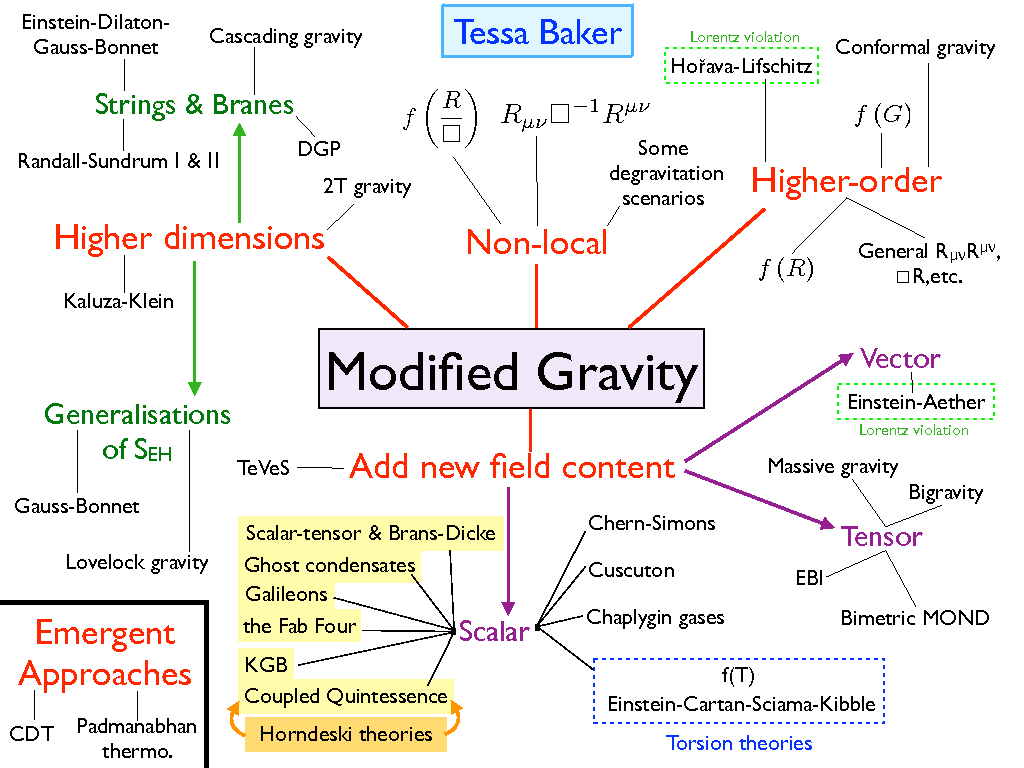
\includegraphics[width=0.7\textwidth]{ModifiedGravity.png}
\bicaption{修改引力理论}
  {Theories of modified gravity. Credit: http://www.cgc-yzu.cn/Upload/research/MG-20240317524.png}
\label{fig:ModGrav}
\end{figure}

从Einstein至今,引力理论已经有了长足的发展,如图\ref{fig:ModGrav}所示,仅基于\GR 基础上发展起来的修改引力理论就已不计其数。
由于和量子力学原理的深刻矛盾,有理由认为Einstein决定论性的的\GR 在某个地方一定背离了引力的物理本质。
然而,时至今日,Einstein昔日基于\GR 所作出的诸多预言,一一被实验所验证;所有可靠的实验检验下,\GR 均可以给出解释——而它通常是最简洁的那个理论。
因此,即使将来的实验证明了\GR 与引力的物理本质之间的偏离,对\GR 的理解依然有着重要的意义。

\section{相对性原理(Principle of relativity)}

\subsection{Galilean相对论}
虽然在20世纪,相对论一次专指Einstein的理论,但是相对性原理(Principle of relativity)的思想在Newtonian力学中就有体现:两个服从Newtonian力学的、相对均匀运动的惯性参考系,无法通过在内部展开的力学实验进行区分。
这一思想一般认为是Galileo在《关于Ptolemaic和 Copernican两大世界体系的对话》中首先提出的\cite{Fang:2012blog}:
\begin{myprop}{Dialogo sopra i due massimi sistemi del mondo}{Dialogo}
把你和一些朋友关在一条大船的甲板下的主舱里,让你们带着几支苍蝇、蝴蝶和其他小飞虫,舱内放一只大碗,其中有几条鱼,然后,挂上一个水瓶,让水一滴一滴地滴到下面的一个宽口罐里。船停着不动时,你留神观察,小虫都以等速向舱内各方向飞行,鱼向各方向随便游动,水滴滴进下面的罐中。你把任何东西扔给你的朋友时,只要距离相等,向这一方向也不比向另一方向更多用力。你的双脚齐跳,无论向哪个方向跳过的距离都相等。当你仔细观察这些事情之后,再使船以任何速度前进,只要运动是均匀的,也不忽左忽右地摆动,你将发现,所有上述现象都没有丝毫变化,你无法从任何一个现象来确定,船是在运动还是在停着不动。即使船运动得相当快,在跳跃时,你也将和以前一样,你跳向船尾也不会比跳向船头更省力。
\end{myprop}
在Galilean相对性原理表明的这个表述中,日常生活中涉及到的物理学性质,在地球坐标系下(船停着不动)和船的坐标系下(船在运动)没有任何区别。

用公式来表述的话,则可以设立两个坐标系,亦即“静止的”地球坐标系S(t,x,y,z)和“运动的”船坐标系S'(t',x',y',z')。
不妨令$t=t'=0$时,两个坐标系重合,且船以速度v沿x方向移动,则有
\begin{equation}
\begin{array}{r@{}l}
t' &{}= t \\
x' &{}= x-vt\\
y' &{}= y \\
z' &{}= z 
\end{array}\label{eq:galileo}
\end{equation}
这种变换通常被称为Galilean变换。

实际上,这种朴素的相对论性原理是非常直观的,在《尚书纬·考灵曜(y{\` a}o)》中,就有文字表达了相当类似的想法:
\begin{myprop}{尚书纬·考灵曜}{Wei}
地恒动不止而人不知,譬如人在大舟中,闭牖(y{\v o}u)而坐,舟行而不觉也
\end{myprop}

\subsection{Maxwell方程组}
通过对电与磁的性质的研究,Maxwell总结了一组著名的方程,用以描述电磁场的一般性质。
在真空中,可以记为
\begin{equation}
\begin{array}{r@{}l}
\nabla \cdot \mathbf {E} &{}= {\frac {\rho }{\varepsilon _{0}}}\\
\nabla \cdot \mathbf {B} &{}= 0\\
\nabla \times \mathbf {E}&{}=-{\frac {\partial \mathbf {B} }{\partial t}}\\
\nabla \times \mathbf {B}&{}=\mu _{0}\left(\mathbf {J} +\varepsilon _{0}{\frac {\partial \mathbf {E} }{\partial t}}\right)
\end{array}\label{eq:maxwell}
\end{equation}
其中$\varepsilon_0$为真空电容率,$\mu_0$为真空磁导率。

Maxwell注意到,通过Maxwell方程组,可以推导出,
\begin{equation}\label{eq:EMwave}
\nabla ^2 \mathbf {B} - \varepsilon_{0} \mu_0 \frac {\partial^2 \mathbf {B} }{\partial^2 t}= 0
\end{equation}
不难看出,电磁场的变化以波动形式传播,其速度$c$取决于:
\begin{equation}\label{eq:SpeedOfLight}
c^2 = \frac{1}{\varepsilon_0 \mu_0}
\end{equation} 
从数值上,$c$的取值与当时已经从实验上测得的光速极为接近,这使得他大胆假设:光就是一种电磁波。

然而,Maxwell方程组与Galilean变换是不自洽的。
考虑在运动的船S'上进行电磁学测量,根据Galilean变换\ref{eq:galileo},电磁场的传播方程\ref{eq:EMwave}变为

\begin{equation}
c^2\nabla^2 \textbf B = \frac{\partial^2 \textbf B}{\partial t^2} + (\textbf v \cdot \nabla)^2 \textbf B - 2 \textbf v \cdot \nabla \left(\frac{\partial \textbf B}{\partial t}\right)
\end{equation}

一个平庸的结论是,通过Galilean变换,船上的物理学家将测得光速变为$c\pm v$。
然而更深刻的问题是,这一结论意味着,如果Galilean相对论是正确的,那么Maxwell方程组只能对某个特定惯性参考系成立,而物理学家可以根据电磁场的测量来确定实验室位于“船”上还是相对静止。
Newtonian力学必须借助绝对绝对空间的概念,在坚持Galilean相对论的前提下,似乎可以得出,满足\ref{eq:EMwave}的参考系就是Newtonian力学概念中的绝对空间。

其时,人们认为电磁波传播需要介质,而这种依附于绝对空间而具有独特性质的参考系,具象化为“以太(aether)”\cite{Yu:EleDyn1997}。

\subsection{\SR}
Lorentz 和Poincar{\'e}第一次意识到,如果S坐标系和S'坐标系之间的转换关系采用如
\begin{equation}
\begin{array}{r@{}l}
t'&{}=\gamma \left(t-{\frac {vx}{c^{2}}}\right)\\
x'&{}=\gamma \left(x-vt\right)\\
y'&{}=y\\
z'&{}=z\\
  \gamma &{}= \frac{1}{{\sqrt {1-v^{2}/c^{2}}}}
\end{array}\label{eq:lorentz}
\end{equation}
的形式的话,那么Maxwell方程组(公式\ref{eq:maxwell})在所有的惯性系中都能成立。
这里的$\gamma$通常被称为Lorentz因子。
形如公式\ref{eq:lorentz}的变换称为Lorentz变换(Lorentz transformation),我们可以说,Maxwell方程组在不同的惯性系中,通过Lorentz变换维持了不变性。

从某种意义上说,Lorentz变换就是\SR 的精髓。
但物理学界今天达成共识,认为是Einstein而非Lorentz或Poincar{\'e}发明了狭义相对论,这是因为Einstein第一次严肃地认为Lorentz变换体现了时间与空间的本质,而非简单的数学玩具。
由此,时间与空间并非完全独立,而是交织在一起,甚至可以互换。
要标记一个事件,必须同时标记其在某个惯性系下的空间坐标(x,y,z)和时间坐标t。
对于两个事件,在S坐标系下看来可能是同时发生的($\Delta t=0$),但在S'坐标系看来却可能发生于不同时间($\Delta t \neq 0$)。
在不同的惯性系下,通过Lorentz变化,两个不同事件之间,保持不变的,是事件间时间间隔和空间间隔的某种组合,称为时空间隔离:
\begin{equation}\label{eq:STinterval}
  \Delta s^2 = - (c\Delta t)^2+ \Delta x ^2 + \Delta y^2+ \Delta z^2
\end{equation}
通常其微分形式使用起来更为方便:
\begin{equation}\label{eq:STinterval_diff}
  {\rm d}s^2 = - (c{\rm d}t)^2+ {\rm d}x ^2 + {\rm d} y^2+ {\rm d} z^2
\end{equation}
在Lorentz变换下,${\rm d}s^2$保持不变。

\section{微分几何初步}
\subsection{张量(tensor)初步}\label{sec:tensor}
在相对论框架下,时间坐标t和空间坐标(x,y,z)联合起来形成一个统一的时空坐标
$x^{\alpha} = (ct,x,y,z)$。
如此处的$\alpha$一般出现在坐标上标上的希腊字母,会遍历{0,1,2,3}。
$x^0= ct$的选取是使得所有的坐标都有着相同的空间量纲,而$x^1 =x, x^2 = y, x^3 = z$则代表空间坐标。
这样,我们可以将公式\ref{eq:STinterval_diff}重新表达为
\begin{equation}\label{eq:STinterval_diff_new}
  {\rm d}s^2 = \eta_ {\alpha \beta}{\rm d}x^\alpha {\rm d} x^\beta
\end{equation}
这里,$\eta_ {\alpha \beta}$是一个对角矩阵,
\begin{equation}\label{eq:Minkowski}
  \eta_{\alpha\beta} ={\begin{pmatrix}
                       -1 & 0 & 0 & 0\\
                        0 & 1 & 0 & 0\\ 
                        0 & 0 & 1 & 0\\
                        0 & 0 & 0 & 1\end{pmatrix}}
\end{equation}
注意到$\eta_{00} = -1$, 而$\eta_{11} = \eta_{22} = \eta_{33} = 1$,并且,根据{\textbf{Einstein 求和约定(Einstein summation convention)}},如公式\ref{eq:STinterval_diff_new}一般,当某个希腊字母同时出现在上下标的时候,则意味着要对该字母求和。
\begin{remark}
  通常,约定俗成:采用希腊字母时,默认遍历\{0,1,2,3\};采用英语字母时,默认遍历\{1,2,3\},即只包含空间项。
\end{remark}

\begin{myprop}{Kronecker delta}{Kronecker}
  有一个特殊的张量,即所谓Kronecker delta张量
\begin{equation}\label{eq:Kronecker}
  \delta_{\alpha\beta} ={\begin{pmatrix}
                        1 & 0 & 0 & 0\\
                        0 & 1 & 0 & 0\\ 
                        0 & 0 & 1 & 0\\
                        0 & 0 & 0 & 1\end{pmatrix}}
\end{equation}
  该张量的表现形式在所有的坐标系中都一致。
\end{myprop}

在更一般的情形下,可以写成
\begin{equation}\label{eq:metric}
  {\rm d}s^2 = g_{\alpha \beta}{\rm d}x^\alpha {\rm d} x^\beta
\end{equation}
我们通常把$\eta_ {\alpha \beta}$称为Minkowski时空中的{\textbf{度规张量}}(metric tensor,在数学语境中通常翻译为度量张量,或者简称为Minkowski度规。
度规张量在Lorentz变换下,遵从一定的变换规则,使得公式\ref{eq:STinterval_diff_new}维持不变量。
也就是说,通过公式\ref{eq:STinterval_diff_new},我们可以把随坐标变换而改变的${\rm }x^{\alpha} $ 转化成不随坐标变换而改变的时空间隔${\rm d} s^2$。\footnote{注意,度规张量是对称的,也就是$g_{\alpha\beta}=g_{\beta\alpha}$。}

可以定义在坐标系中的矢量${\rm d}\vec{x} = \vec{e}_\alpha {\rm d}x^\alpha$。
在坐标系变换过程中,由于坐标基底$\vec{e}_\alpha = \partial \vec{x}/ \partial x^\alpha$改变了,相应的矢量${\rm d}\vec{x} $在坐标基底上的分量${\rm d}x^\alpha$也会变化,但是矢量本身${\rm d}\vec{x} $是不变的
\footnote{注意,在非Euclidean 几何中,指标的上下具有特定的含义,上指标如$x^\alpha$对应于矢量,而下指标如$\vec{x}_\alpha$对应于所谓(1-形式)one-form,有时候也称对偶矢量。
感兴趣的读者请自行参阅\GR 方面的参考资料,在本书中恕不详细展开。}
需要指出的是,矢量也是一种张量。
实际上,张量也符合上述性质:当坐标基底改变时,张量在坐标基底上的分量会发生变化,但是张量本身是不变的。

度规也自然地定义了在坐标系中两个矢量的内积。
${\rm d}\vec{x}$与自己的内积是时空间隔${\rm d}s^2$,展开得:
\begin{equation}\label{eq:InnerProduct1}
  {\rm d}s^2 =  {\rm d}\vec{x}\cdot{\rm d}\vec{x} = \left(\vec{e}_\alpha \cdot \vec{e}_\beta \right) {\rm d}x^\alpha {\rm d}x^\beta
\end{equation}
通过与公式\ref{eq:metric}比较,可以发现$g_{\alpha\beta} = \vec{e}_\alpha \cdot \vec{e}_\beta$。
更一般的,两个矢量$\vec{A} = A^\alpha \vec{e}_\alpha$和$\vec{B} = B^\alpha \vec{e}_\alpha$的内积可以写成
\begin{equation}\label{eq:InnerProduct2}
  \vec{A}\cdot\vec{B}= A^\alpha B^\beta \left(\vec{e}_\alpha \cdot \vec{e}_\beta \right) =  g_{\alpha \beta}A^\alpha B^\beta.
\end{equation}

\subsection{等效原理}
Einstein的\SR,虽然可以将牛顿框架下的绝对空间观点移除,但惯性系仍然在所有的坐标系中占据一个特殊的位置。\footnote{扩展阅读:\cite{Rindler:GR}等著作中关于Mach's principle和Isaac Newton's rotating bucket argument (also known as Newton's bucket)的讨论。}
由此探究了十年时间之后,Einstein最终得到了\GR ,并最终将惯性系的特殊性也彻底移除。
Einstein观察到,在Newtonian力学体系中,质量$m$这个概念出现在两个完全截然不同的地方:Newton's second law of motion 指出,物体所受的力$F=ma$,这里$a$为加速度,由此可以定义出惯性质量$m_I$。
而在万有引力波公式中,Newton又指出,物体所受的引力与其质量大小成正比,由此定义了引力质量$m_G$。
两者的语境完全不同,而实验可以证明在实验精度内$m_I = m_G$精确成立。
两种质量的严格相等,通常被称为“弱”等效原理。\footnote{需要注意,弱等效原理的表述方式有很多,但是几种表述互相之间均等效。}

拥有相同质量的物体,可以拥有完全不同的电量,由此在电场中受到不同的电磁力作用。
然而拥有相同惯性质量$m_I$的物体,一定拥有相同的引力质量$m_G$,这也就暗示了引力作用从本质上和其他相互作用的区别。
在\SR 的语境中,物理学家无法通过任何局部开展的实验了解自己所处的船舱是否处于均匀运动状态。
而弱等效原理中,物理学家无法通过实验分辨船舱是在加速(由$m_I$确定,服从Newton's second law of motion)还是受到了引力作用(由$m_G$确定,服从引力作用)。 既然加速度和引力等价,那么处于自由下落状态的实验室,所开展的所有{\textbf{局域(local)}}实验结果,都将完全一样,这一点与实验室的速度、所处的位置都不相关。
这一等价性,被称为“强”等效原理。\cite{Schutz:FirstCourse}

根据强等效原理,所有在局域展开的物理实验,只要转换到自由落体状态的参考系下看,都是一致的。
换言之,可以将自由落体参考系下的结果,通过合理的坐标变换,得到有引力时的表达式。
最重要的,就是度规的转换。
在自由落体状态时候,局部Lorentz坐标系$\xi^\mu$遵从Minkowski度规$\eta_{\mu\nu}$。
假设一般的坐标系$x^\alpha$与局部Lorentz坐标系之间符合转换关系$\xi ^\mu= f^\mu (x^\alpha)$,则有 ${\rm d} \xi ^\mu = (\partial_\alpha f^\mu) {\rm d}x^\alpha$。
可以得到 
\begin{equation}\label{eq:STinterval_diff_GR} 
  {\rm d}s^2 = \left( \eta_ {\mu \nu} \partial_\alpha f^\mu \partial_\beta f^\nu\right){\rm d} x^\alpha {\rm d} x^\beta
\end{equation}
与公式\ref{eq:metric}比较,可以得到,
$g_{\alpha\beta} = \eta_ {\mu \nu} \partial_\alpha f^\mu \partial_\beta f^\nu$

\begin{myprop}{Raising and Lowering of index}{RaiseLower}
  指标的上下标具有不同的含义。
  对于一维的张量而言,指标在上时是{\textbf{矢量}},其坐标转换关系满足逆变(contravariant);指标在下时是{\textbf{对偶矢量}}(或1-形式),其坐标转换关系满足协变(covariant)。
  指标可以通过度规$g_{\mu\nu}$进行升降。
  首先可以定义逆变张量$g^{\mu\nu}$
\begin{equation}\label{eq:RaiseLower} 
  g^{\alpha\mu} g_{\mu\beta}=  \delta^{\alpha}_{\beta}
\end{equation}
  其中$\delta^{\alpha}_{\beta}$是Kronecker delta张量,数值上与公式\ref{eq:Kronecker}一致。
  利用度规,可以实现指标的升降:
\begin{equation}\label{eq:Raise} 
  A^\alpha = g^{\alpha\beta} A_{\beta}  
\end{equation}
类似地,有
\begin{equation}\label{eq:Lower} 
  A_{\beta}= g_{\beta\alpha}  A^\alpha .
\end{equation}

\end{myprop}


\subsection{协变导数} 
Minkowski度规描述的是平直时空,而所有非Minkowski度规对应的都是弯曲时空。
因此在\GR 的框架下,要描述动力学,就需要运用弯曲的时空对应的数学语言,或者是非Euclidean几何(non-Euclidean geometry)
\begin{figure}[htp]
\centering
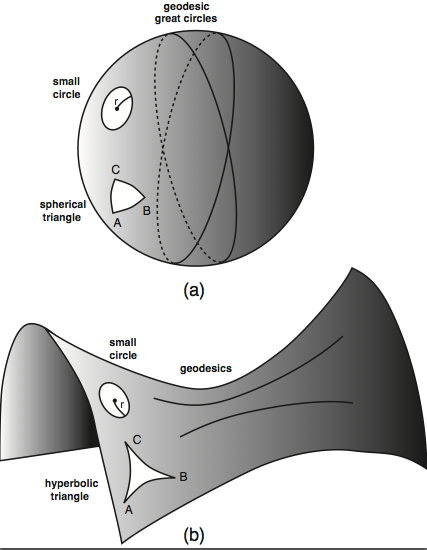
\includegraphics[width=0.5\textwidth]{Two-noneuclidean-surfaces.jpg}
\bicaption{两个非Euclidean 几何的例子}
  {two examples of non-Euclidean geometry. Credit: https://blogs.futura-sciences.com/e-luminet/2017/09/22/non-euclidean-geometries/}
\label{fig:nonEuclidean}
\end{figure}

\begin{myprop}{Parallel postulate}{ParallelPostulate}
  Euclidean几何的五大公设中,第五公设为:

  {\textbf{若两条直线都与第三条直线相交,并且在同一边的内角之和小于两个直角,则这两条直线在这一边必定相交。}}。

  这一定义相较其他公设更为冗长,并不是那么显然。
  晚近的研究表明,将第五公设去除后,也可以构成自洽的几何体系,即所谓非Euclidean几何。
  根据曲率的不同,可以将其分为椭圆几何(又称Riemannian 几何,任意两条直线一定相交;三角形内角和小于$180^\circ$)和双曲几何(又称Lobachevskian几何,至少可以引出两条平行线;三角形内角和大于$180^\circ$)。
\end{myprop}

对于函数$\vec{A}(x)$的导数,我们通常定义为$\lim_{{\rm d}x \to 0}\frac{\vec{A}(x+{\rm d}x)-\vec{A}(x)}{{\rm d}x}$。
然而在非Euclidean几何中,需要重新审视一些在Euclidean几何里习以为常的概念:比如,{\textbf{矢量}}的定义必须依赖局部的坐标系。
如此一来,$\vec{A}(x+{\rm d}x)-\vec{A}(x)$的具体取值,就很值得玩味:如何对不在同一个位置处的两个矢量进行比较?

在Euclidean几何中这并不是一个问题,因为可以简单的平移矢量$\vec{A}(x)$至$x+{\rm d}x$处,然后与$\vec{A}(x+{\rm d}x)$比较。
然而,在非Euclidean几何中,矢量的平移这个概念也需要被仔细检阅。
具体来说,平移后的矢量,不仅取决于矢量的指向,也取决于平移的路径。

\begin{example}

让我们想象一个生活在地球仪表面的二维生物(不妨假设这是一个没有厚度的蚂蚁,它只能沿着地球仪表面运动),假设这只蚂蚁从地球仪上的$(0^\circ,0^\circ)$出发(也就是本初子午线和赤道的交点),决心一路向北。

在任意时刻,它的前进方向都是一个矢量,在起点处,这个方向指向正北。
随着它的运动,这个矢量被不断的平移(注意,在这个二维球面空间里,矢量也只能在地球仪表面上定义)。
当它到达北极点时,这个平移后的矢量就称为指向东西经$180^\circ$线。
在我们的三维世界里去看的话,会发现,两个矢量的方向其实是垂直的(再继续走1/4圈的话就变成了指向南极方向,与原方向相反了)。
\end{example}

\begin{figure}[htp]
\centering
\includegraphics[width=0.7\textwidth]{CovDeriv.png}
  \bicaption{非Euclidean 几何中矢量协变导数的图示}
  {demonstration of covariant derivative of vectors in non-Euclidean geometry. Credit: Martin Hendry}
\label{fig:CovDeriv}
\end{figure}

如图\ref{fig:CovDeriv}所示,在$P$点处(坐标为$x^\beta$)有一矢量$\vec{A}(x)$,其坐标分量为$A^\alpha$,经过$P \to Q$的路径到达Q点(坐标为$x^\alpha+{\rm d}x^\alpha$),这时,如果保持原来的坐标分量不变,则分量依然是$A^\alpha$。
与Euclidean 几何不同,由于不同点处坐标基底也发生了改变,因此在$x+{\rm d}x$处的$A^\alpha$并不一定与$\vec{A}(x)$平行,真正平行的矢量为$\vec{DA}(x+{\rm d}x)$,其坐标分量为$DA^\alpha$
\begin{equation}\label{eq:parallel}
  DA^\alpha(x+{\rm d}x) = A^\alpha(x) + \delta A^\alpha(x)
\end{equation}
由坐标基底$\vec{e}$发生变化而引起的$\delta A^\alpha$
\begin{equation}\label{eq:deltaA}
  \delta A^\alpha(x) = -\Gamma^\alpha_{~\mu\beta} A^\mu {\rm d}x^\beta
\end{equation}
其中,$\Gamma^\alpha_{~\mu\beta}$是Christoffel符号,通过它,可以得到不同位置处坐标基底之间的转换关系
\begin{equation}\label{eq:Christoffel}
\frac{\partial \vec{e}_\mu}{\partial x^\beta} = \Gamma^\alpha_{~\mu\beta} \vec{e}_\alpha。
\end{equation}

再次强调:我们在\ref{sec:tensor}节中提到过,在坐标基底发生变化时,张量的具体分量会变化,但是张量本身不会变。
当我们定义了矢量的平移以后,我们终于可以合理地定义矢量的(不随坐标基底变化的)导数了:可以在Q点$x+{\rm d}x$处,将$\vec{A}(x+{\rm d}x)$与从P点平移而来的$\vec{DA}(x+{\rm d}x)$进行比较。
这样定义出来的导数,我们称之为协变导数(covariant derivative)$A^\alpha_{~; \beta}$(见图\ref{fig:CovDeriv})。
\begin{equation}\label{eq:CovDeriv}
A^\alpha_{~; \beta} \equiv \lim_{{\rm d}x^\beta \to 0}\frac{\vec{A}^\alpha(x^\beta+{\rm d}x^\beta)-\vec{DA}^\alpha(x^\beta+{\rm d}x^\beta)}{{\rm d}x^\beta} =A^\alpha_{~, \beta} + \Gamma^\alpha_{~\mu\beta}A^\mu
\end{equation}
其中,$A^\alpha_{~, \beta}$是普通的偏导$\partial A^\alpha/\partial x^\beta$。

通过度量张量$g_{\mu\nu}$的协变导数为0,并通过交换指标、求和,可以得到
\begin{equation}\label{eq:ChristoffelDef}
\Gamma ^{\mu}_{{~\alpha\beta}}={\frac  {1}{2}}g^{{\mu\nu}}\left({\frac  {\partial g_{{\nu\alpha}}}{\partial x^{\beta}}}+{\frac  {\partial g_{{\nu\beta}}}{\partial x^{\alpha}}}-{\frac  {\partial g_{{\alpha\beta}}}{\partial x^{\nu}}}\right),
\end{equation}
这里可以看出,不同局部之间的联系,完全由局部的度规决定。

\subsection{测地线(geodesics)}
我们关心一个粒子的世界线\footnote{世界线是三位空间中“轨迹”概念的延生和对应。},每一个原时(proper time)$\tau$的取值都可以对应一个坐标点$x^\alpha$,同时有${\rm d}\tau = \sqrt{-{\rm d}s^2}/c$。
可以定义,在$x^\alpha$处,粒子运动的速度(切矢)为
\begin{equation}\label{eq:velocity}
  u^\alpha = \frac{{\rm d}x^\alpha}{{\rm d}\tau},
\end{equation}
不难得到
\begin{equation}\label{eq:gmunuNorm}
  g_{\alpha \beta}u^\alpha u^\beta = c^2  
\end{equation}

Newtonian力学描述物体在惯性系中沿直线运动。
然而,在弯曲时空中,直线的概念消失了;而和直线概念最为接近的,就是测地线。
我们考虑一条曲线,它的每一个点上的切矢都与前一个点上的切矢平行,这样的操作可以唯一定义一条曲线,这样的曲线叫做测地线。
根据定义,则有
\begin{equation}\label{eq:ParaTrans}
  \frac{{\rm d}\vec{u}}{{\rm d}\tau}=0
\end{equation}
代入速度定义式\ref{eq:velocity}和协变导数公式\ref{eq:CovDeriv},可以得到
\begin{equation}\label{eq:geodesics}
  \frac{{\rm d}^2 x^\mu}{{\rm d}\tau^2}+ \Gamma^\mu_{~\alpha\beta}\frac{{\rm d}x^\alpha}{{\rm d}\tau}\frac{{\rm d}x^\beta}{{\rm d}\tau}=0
\end{equation}
这样一条测地线描述了在\GR 框架下,Newton's second law of motion的对应:不受外力作用的物体,沿测地线运动。
需要特别说明的是,在推导过程中,我们默认了类时的测地线,这样,每一个点对应一个原时$\tau$。
然而,对于类光的测地线(即,测地线上每一点的原时$\tau$都相同),将$\tau$替换成仿射参量(affine parameter)$\lambda$以后,公式\ref{eq:ParaTrans}依然成立。
特别的,这样的测地线称为{\textbf{零测地线(null geodesics)}}。

\section{\GR (General Relativity)初步}
\subsection{曲率张量}
我们之前说过,在非Euclidean 几何中,三角形内角和不等于$180^\circ$,但显然三角形需要三个顶点,并不一定能在某个足够小的局域定义。
能不能通过对某个点的时空性质观察,局域地确定时空是否弯曲?
答案是肯定的,借助的工具就是Riemann 张量。
\begin{equation}\label{eq:RiemannTensor}
  R^\alpha_{~\beta\gamma\delta}= \partial_\gamma \Gamma^{\alpha}_{~\beta \delta}- \partial_\delta\Gamma^{\alpha}_{~\beta \gamma }+\Gamma^{\alpha}_{~\mu \gamma }\Gamma^{\mu}_{~\beta \delta }-\Gamma^{\alpha}_{~\mu \delta }\Gamma^{\mu}_{~\beta \gamma } 
\end{equation}
各类对称性可以消除独立分量的数目,在四维时空中,Riemann 张量一共有20个独立分量。

在Riemann 张量基础上,还可以定义两个重要的张量:Ricci张量
\begin{equation}\label{eq:RicciTensor}
  R_{\alpha\beta} \equiv R^\mu_{~\alpha\mu\beta}
\end{equation}
和Einstein张量
\begin{equation}\label{eq:EinsteinTensor}
  G_{\alpha\beta} \equiv R_{\alpha\beta} -\frac{1}{2}g_{\alpha\beta}R.
\end{equation}
其中$R =g^{\alpha\beta}R_{\alpha\beta}$。

\subsection{Einstein场方程}

可以证明\footnote{可以通过Bianchi恒等式证明,具体过程请参阅各参考书。},
\begin{equation}\label{eq:ConBianIden}
  G^{\alpha\beta}_{~~;\beta} =0.
\end{equation}
上述等式有时被称为缩并Bianchi恒等式。

在Newtonian引力中,
\begin{equation}\label{eq:NewtonPoisson}
  \nabla ^2 \left(-\frac{Gm}{r}\right) = 4\pi G \rho
\end{equation}
等式的左边描述引力势(通常由$\Phi$表示),等式的右边描述的是质量分布。
在\GR 下,虽然对引力的描述改变了,Einstein认为引力是时空弯曲的表现,所以上述等式中的左边可以对应于$G_{\alpha\beta}$,而质量分布在相对论中的对应是所谓能量-动量张量$T_{\alpha\beta}$\footnote{有时候称为应力-能量张量,也称应力-能量-动量张量、能量-应力张量}。
\begin{figure}[htp]
\centering
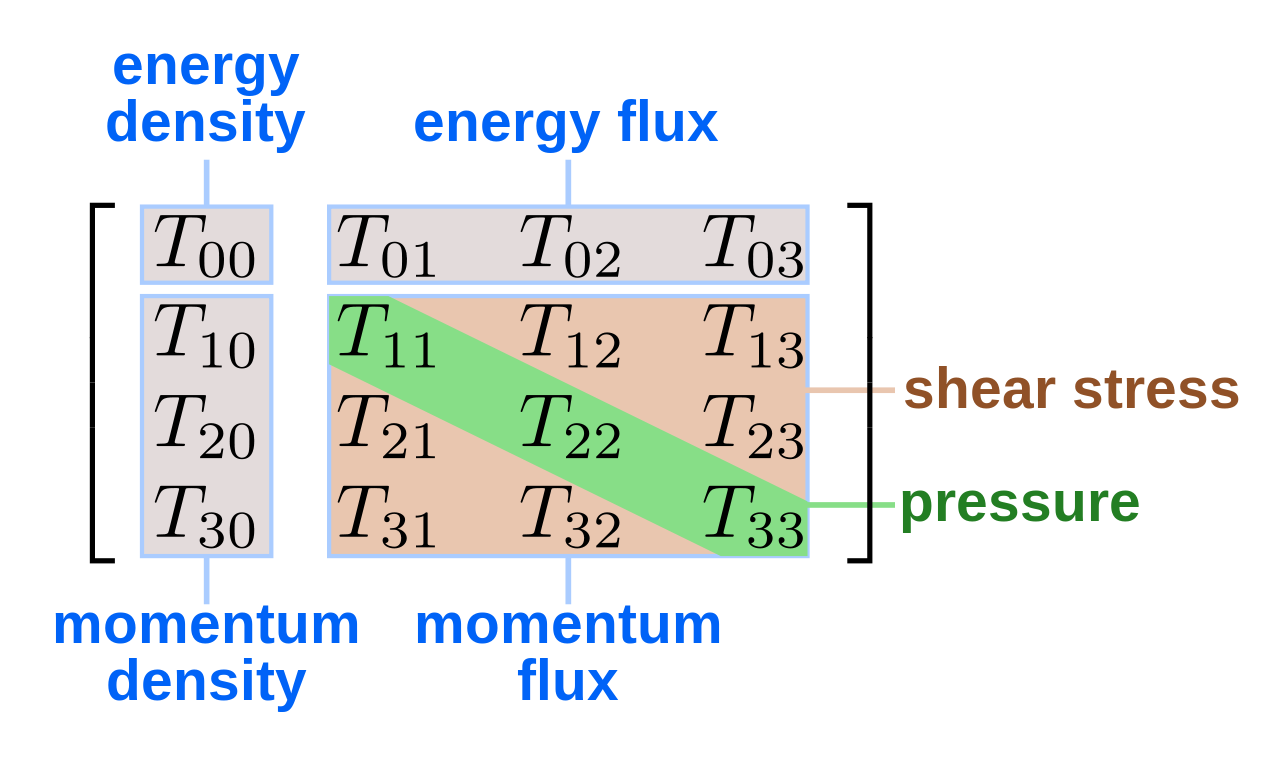
\includegraphics[width=0.7\textwidth]{StressEnergyTensor.png}
\bicaption{能量-动量张量的协变分量}
  {Covariant components of the energy-momentum tensor Credit: https://commons.wikimedia.org/wiki/File:StressEnergyTensor.svg}
\label{fig:Tmunu}
\end{figure}
$T^{\alpha\beta}$是$\alpha$方向的动量流穿越等$x^\beta$线的分量。
对于理想流体而言,$T^{00}$是能量密度,$T^{ii}$是压强,其他分量皆为零。
由连续性要求可以得到
\begin{equation}\label{eq:Continuity}
  T^{\alpha\beta}_{~~;\beta} =0.
\end{equation}
 
面对公式\ref{eq:ConBianIden}和公式\ref{eq:Continuity},Einstein猜测其解的形式为
\begin{equation}\label{eq:FieldEq1}
  G^{\alpha\beta} =kT^{\alpha\beta}
\end{equation}
通过在弱场情形下与Newtonian引力的比较,可以确定常数k的取值,
\begin{equation}\label{eq:FieldEq2}
  G^{\alpha\beta} =\frac{8\pi G}{c^4}T^{\alpha\beta}
\end{equation}
这就是\GR 中描述时空与质量分布关系的公式为Einstein场方程。

\begin{myprop}{Summerize of GR}{GRoneLine}
John Wheeler 关于\GR 有一段非常著名的总结:\\
The matter tells spacetime how to curve, and the spacetime tells matter how to move\\
  结合上述公式来看,可以看到,Einstein场方程(公式\ref{eq:FieldEq2})告诉了时空如何根据质量分布而弯曲;而连续性方程(公式\ref{eq:Continuity})告诉了质量如何运动。
\end{myprop}
